\documentclass[,a4paper,12pt,french]{article}

\usepackage{../../Style}
\pagestyle{empty}

% Début du document
%%%%%%%%%%%%%%%%%%%
\begin{document}

\vfill

\compo[0.5]
{
\begin{center}
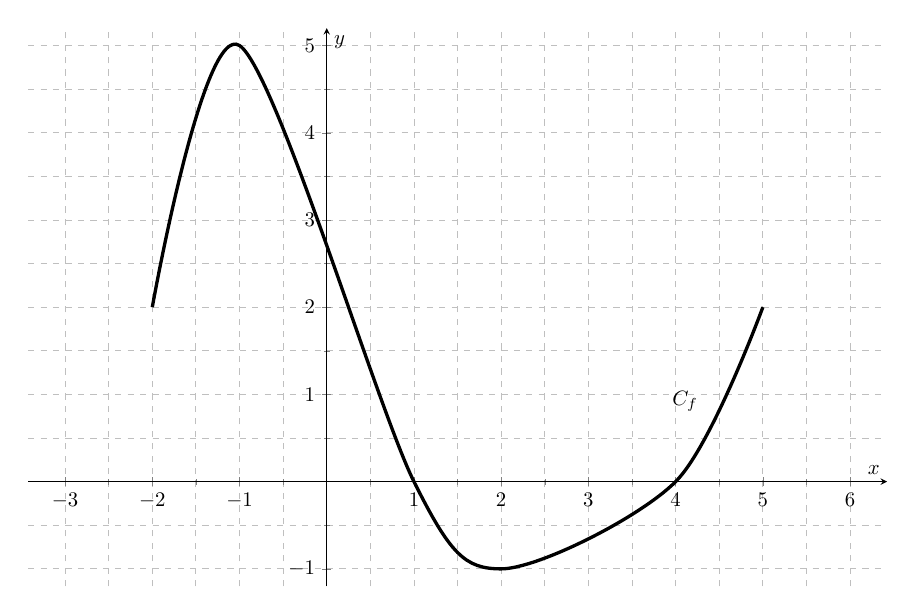
\begin{tikzpicture}[scale=0.75]
\begin{axis}[
axis x line=bottom,
axis y line = left,
axis lines=middle,
width=1.33\linewidth,
height=0.91\linewidth,
xmin=-2, xmax=5,
ymin=-1, ymax=5,
enlargelimits={abs=0.2},
xlabel={$x$},
ylabel={$y$},
minor x tick num=1,
minor y tick num=1,
%ytick distance=1,
grid=both,
grid style=dashed,
axis equal,
legend pos=north east
]
\addplot[samples=101,smooth,ultra thick,domain=(0:4),mark=none] plot coordinates {(-2,2) (-1,5) (1,0) (2,-1) (4,0) (5,2)} node [pos=0.9,above left] {$\mathscr C_f$};

\end{axis}
\end{tikzpicture}
\end{center}
}
{
\begin{center}
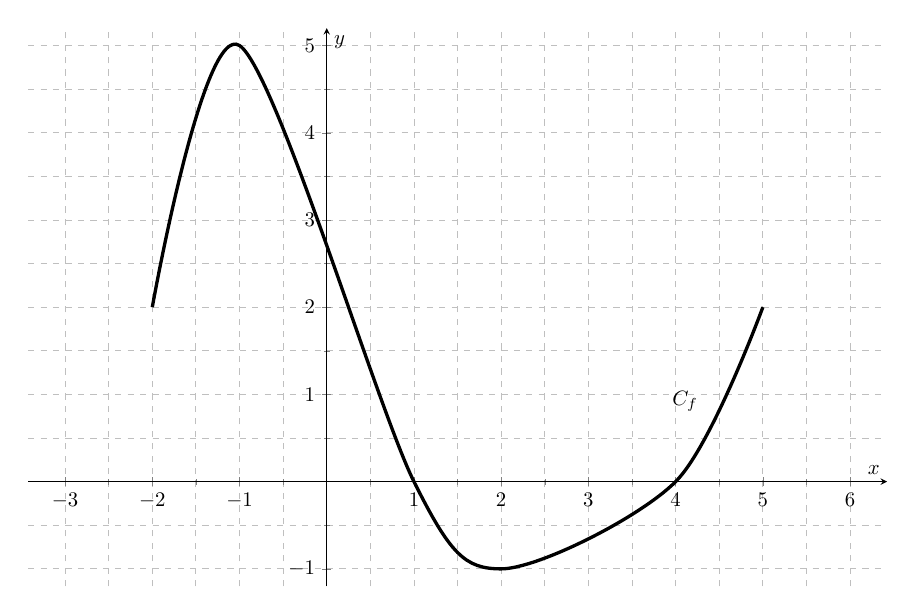
\begin{tikzpicture}[scale=0.75]
\begin{axis}[
axis x line=bottom,
axis y line = left,
axis lines=middle,
width=1.33\linewidth,
height=0.91\linewidth,
xmin=-2, xmax=5,
ymin=-1, ymax=5,
enlargelimits={abs=0.2},
xlabel={$x$},
ylabel={$y$},
minor x tick num=1,
minor y tick num=1,
%ytick distance=1,
grid=both,
grid style=dashed,
axis equal,
legend pos=north east
]
\addplot[samples=101,smooth,ultra thick,domain=(0:4),mark=none] plot coordinates {(-2,2) (-1,5) (1,0) (2,-1) (4,0) (5,2)} node [pos=0.9,above left] {$\mathscr C_f$};

\end{axis}
\end{tikzpicture}
\end{center}
}

\vfill

\compo[0.5]
{
\begin{center}
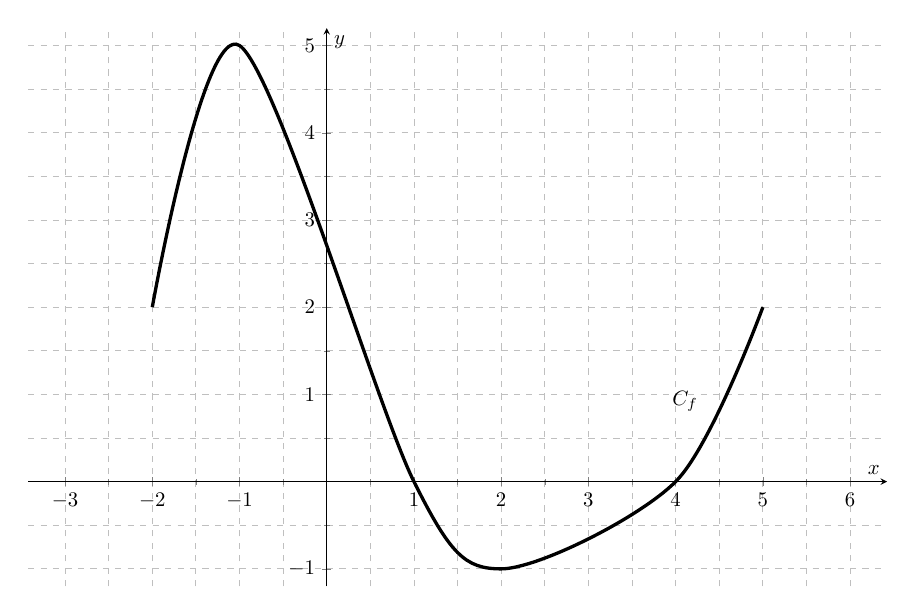
\begin{tikzpicture}[scale=0.75]
\begin{axis}[
axis x line=bottom,
axis y line = left,
axis lines=middle,
width=1.33\linewidth,
height=0.91\linewidth,
xmin=-2, xmax=5,
ymin=-1, ymax=5,
enlargelimits={abs=0.2},
xlabel={$x$},
ylabel={$y$},
minor x tick num=1,
minor y tick num=1,
%ytick distance=1,
grid=both,
grid style=dashed,
axis equal,
legend pos=north east
]
\addplot[samples=101,smooth,ultra thick,domain=(0:4),mark=none] plot coordinates {(-2,2) (-1,5) (1,0) (2,-1) (4,0) (5,2)} node [pos=0.9,above left] {$\mathscr C_f$};

\end{axis}
\end{tikzpicture}
\end{center}
}
{
\begin{center}
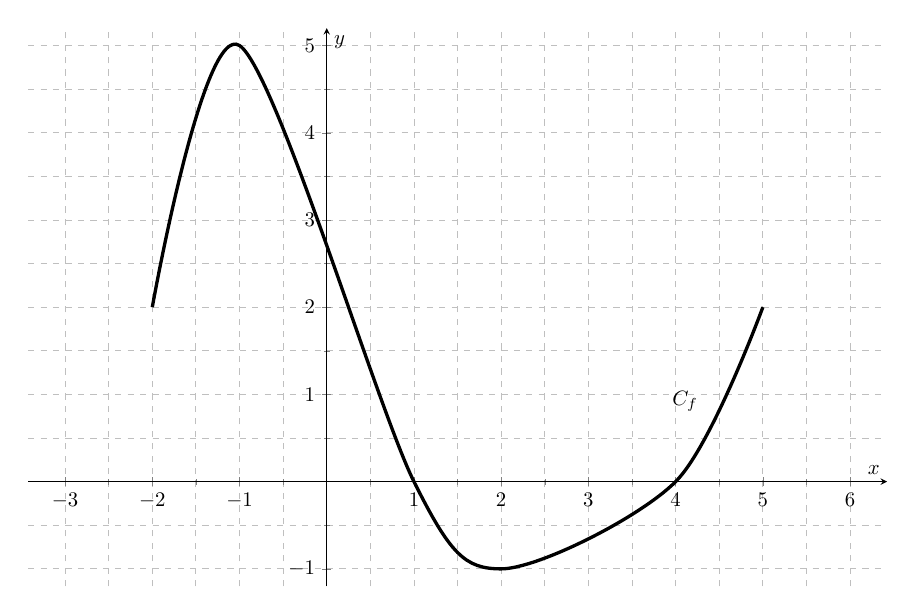
\begin{tikzpicture}[scale=0.75]
\begin{axis}[
axis x line=bottom,
axis y line = left,
axis lines=middle,
width=1.33\linewidth,
height=0.91\linewidth,
xmin=-2, xmax=5,
ymin=-1, ymax=5,
enlargelimits={abs=0.2},
xlabel={$x$},
ylabel={$y$},
minor x tick num=1,
minor y tick num=1,
%ytick distance=1,
grid=both,
grid style=dashed,
axis equal,
legend pos=north east
]
\addplot[samples=101,smooth,ultra thick,domain=(0:4),mark=none] plot coordinates {(-2,2) (-1,5) (1,0) (2,-1) (4,0) (5,2)} node [pos=0.9,above left] {$\mathscr C_f$};

\end{axis}
\end{tikzpicture}
\end{center}
}

\vfill

\compo[0.5]
{
\begin{center}
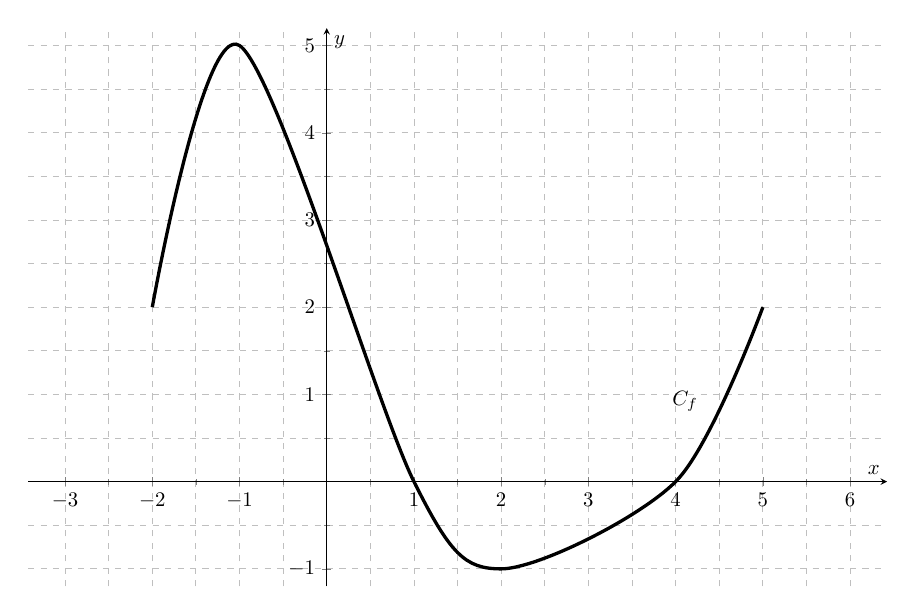
\begin{tikzpicture}[scale=0.75]
\begin{axis}[
axis x line=bottom,
axis y line = left,
axis lines=middle,
width=1.33\linewidth,
height=0.91\linewidth,
xmin=-2, xmax=5,
ymin=-1, ymax=5,
enlargelimits={abs=0.2},
xlabel={$x$},
ylabel={$y$},
minor x tick num=1,
minor y tick num=1,
%ytick distance=1,
grid=both,
grid style=dashed,
axis equal,
legend pos=north east
]
\addplot[samples=101,smooth,ultra thick,domain=(0:4),mark=none] plot coordinates {(-2,2) (-1,5) (1,0) (2,-1) (4,0) (5,2)} node [pos=0.9,above left] {$\mathscr C_f$};

\end{axis}
\end{tikzpicture}
\end{center}
}
{
\begin{center}
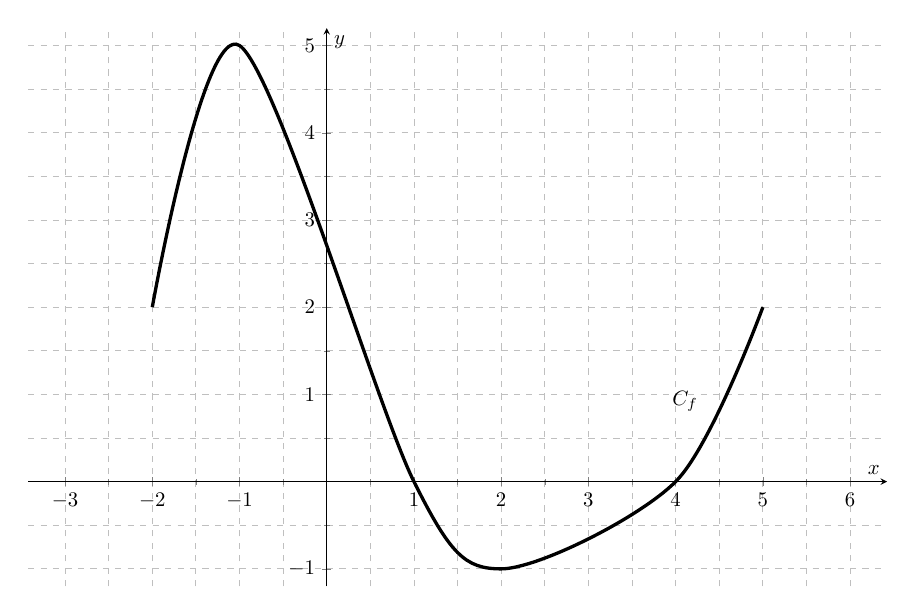
\begin{tikzpicture}[scale=0.75]
\begin{axis}[
axis x line=bottom,
axis y line = left,
axis lines=middle,
width=1.33\linewidth,
height=0.91\linewidth,
xmin=-2, xmax=5,
ymin=-1, ymax=5,
enlargelimits={abs=0.2},
xlabel={$x$},
ylabel={$y$},
minor x tick num=1,
minor y tick num=1,
%ytick distance=1,
grid=both,
grid style=dashed,
axis equal,
legend pos=north east
]
\addplot[samples=101,smooth,ultra thick,domain=(0:4),mark=none] plot coordinates {(-2,2) (-1,5) (1,0) (2,-1) (4,0) (5,2)} node [pos=0.9,above left] {$\mathscr C_f$};

\end{axis}
\end{tikzpicture}
\end{center}
}

\vfill

\compo[0.5]
{
\begin{center}
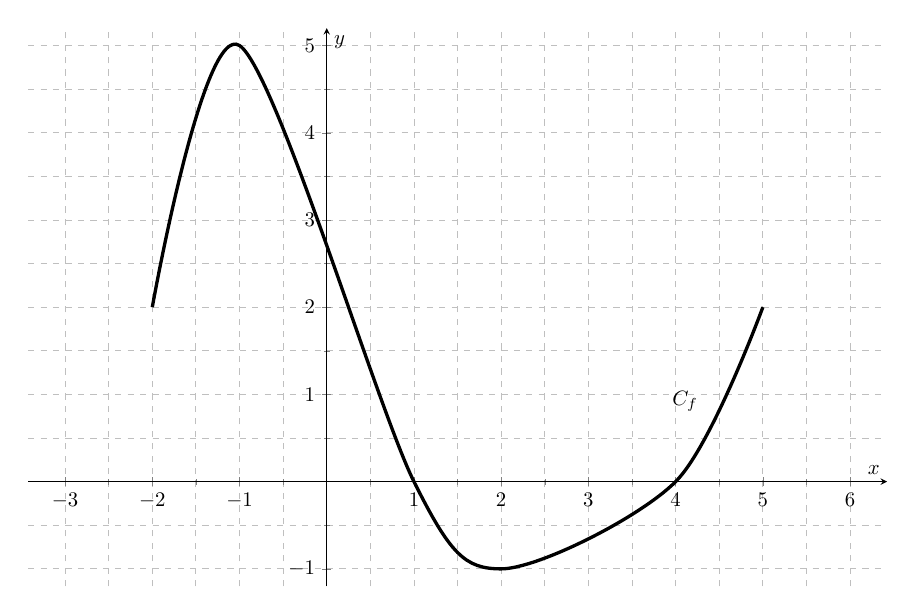
\begin{tikzpicture}[scale=0.75]
\begin{axis}[
axis x line=bottom,
axis y line = left,
axis lines=middle,
width=1.33\linewidth,
height=0.91\linewidth,
xmin=-2, xmax=5,
ymin=-1, ymax=5,
enlargelimits={abs=0.2},
xlabel={$x$},
ylabel={$y$},
minor x tick num=1,
minor y tick num=1,
%ytick distance=1,
grid=both,
grid style=dashed,
axis equal,
legend pos=north east
]
\addplot[samples=101,smooth,ultra thick,domain=(0:4),mark=none] plot coordinates {(-2,2) (-1,5) (1,0) (2,-1) (4,0) (5,2)} node [pos=0.9,above left] {$\mathscr C_f$};

\end{axis}
\end{tikzpicture}
\end{center}
}
{
\begin{center}
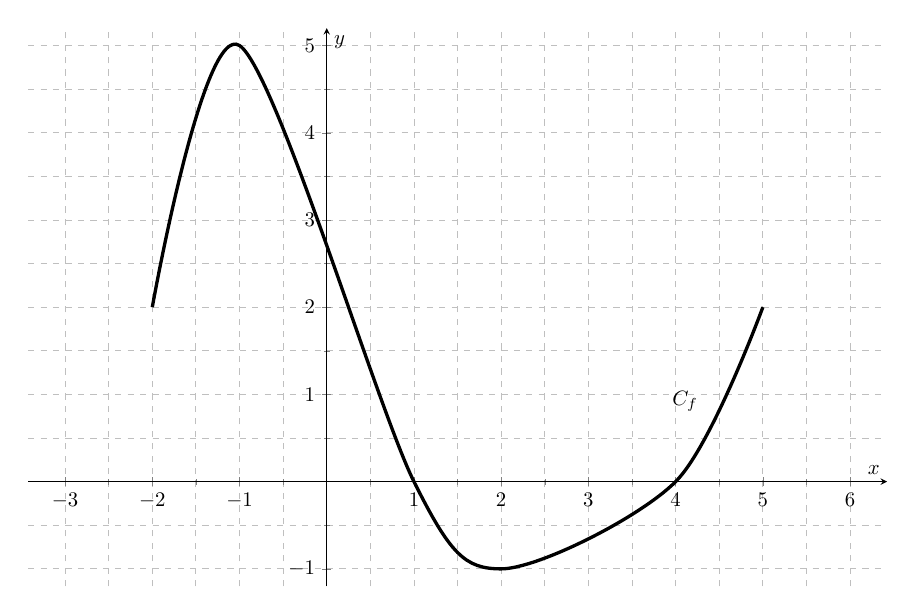
\begin{tikzpicture}[scale=0.75]
\begin{axis}[
axis x line=bottom,
axis y line = left,
axis lines=middle,
width=1.33\linewidth,
height=0.91\linewidth,
xmin=-2, xmax=5,
ymin=-1, ymax=5,
enlargelimits={abs=0.2},
xlabel={$x$},
ylabel={$y$},
minor x tick num=1,
minor y tick num=1,
%ytick distance=1,
grid=both,
grid style=dashed,
axis equal,
legend pos=north east
]
\addplot[samples=101,smooth,ultra thick,domain=(0:4),mark=none] plot coordinates {(-2,2) (-1,5) (1,0) (2,-1) (4,0) (5,2)} node [pos=0.9,above left] {$\mathscr C_f$};

\end{axis}
\end{tikzpicture}
\end{center}
}

\vfill

\compo[0.5]
{
\begin{center}
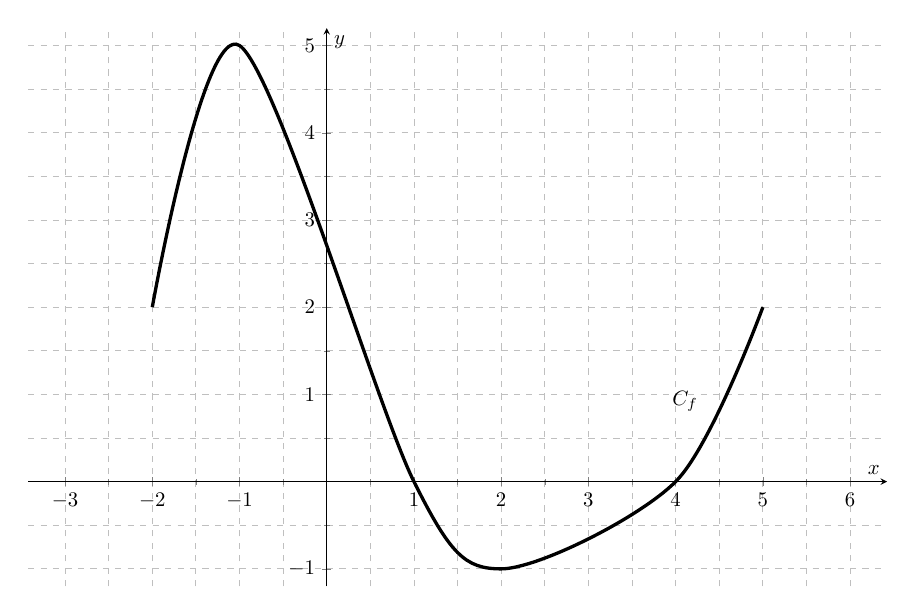
\begin{tikzpicture}[scale=0.75]
\begin{axis}[
axis x line=bottom,
axis y line = left,
axis lines=middle,
width=1.33\linewidth,
height=0.91\linewidth,
xmin=-2, xmax=5,
ymin=-1, ymax=5,
enlargelimits={abs=0.2},
xlabel={$x$},
ylabel={$y$},
minor x tick num=1,
minor y tick num=1,
%ytick distance=1,
grid=both,
grid style=dashed,
axis equal,
legend pos=north east
]
\addplot[samples=101,smooth,ultra thick,domain=(0:4),mark=none] plot coordinates {(-2,2) (-1,5) (1,0) (2,-1) (4,0) (5,2)} node [pos=0.9,above left] {$\mathscr C_f$};

\end{axis}
\end{tikzpicture}
\end{center}
}
{
\begin{center}
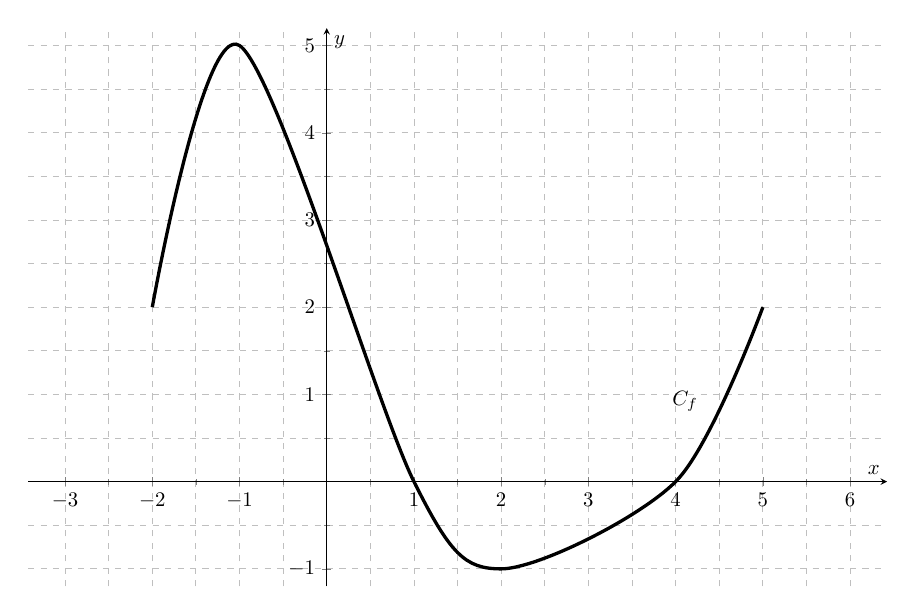
\begin{tikzpicture}[scale=0.75]
\begin{axis}[
axis x line=bottom,
axis y line = left,
axis lines=middle,
width=1.33\linewidth,
height=0.91\linewidth,
xmin=-2, xmax=5,
ymin=-1, ymax=5,
enlargelimits={abs=0.2},
xlabel={$x$},
ylabel={$y$},
minor x tick num=1,
minor y tick num=1,
%ytick distance=1,
grid=both,
grid style=dashed,
axis equal,
legend pos=north east
]
\addplot[samples=101,smooth,ultra thick,domain=(0:4),mark=none] plot coordinates {(-2,2) (-1,5) (1,0) (2,-1) (4,0) (5,2)} node [pos=0.9,above left] {$\mathscr C_f$};

\end{axis}
\end{tikzpicture}
\end{center}
}

\end{document}
